
%(BEGIN_QUESTION)
% Copyright 2010, Tony R. Kuphaldt, released under the Creative Commons Attribution License (v 1.0)
% This means you may do almost anything with this work of mine, so long as you give me proper credit

Et steinknuseanlegg bruker et sett med vannspraydyser for å ``slå ned'' støv som frigjøres når steinene forlater knusemaskinen via en sjakt og ned på et transportbånd:

$$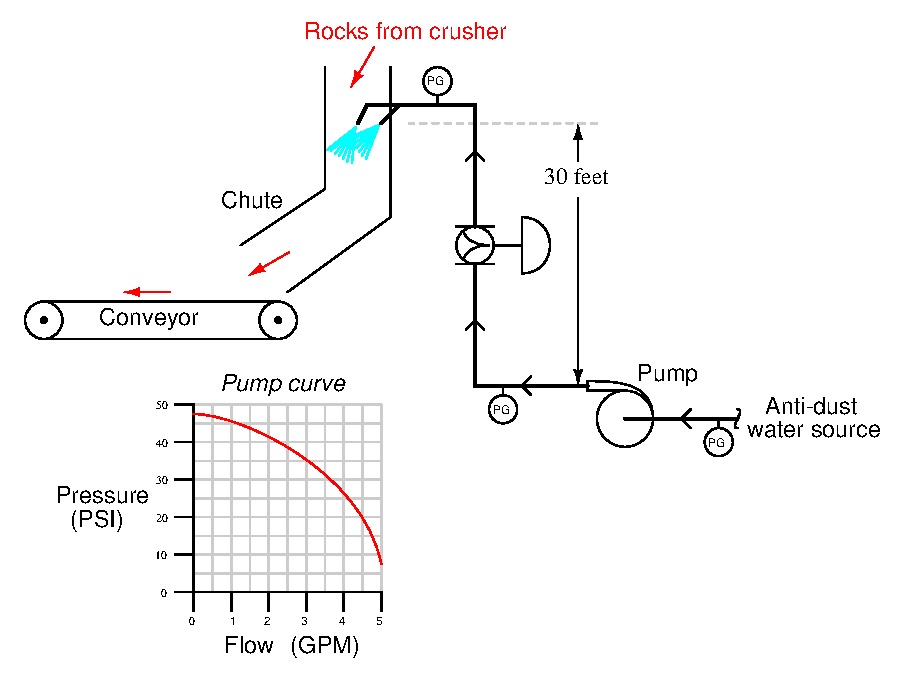
\includegraphics[width=15.5cm]{i01409x01.eps}$$

Bestem nødvendig $C_{v}$-verdi for denne reguleringsventilen for å oppnå en strømningsrate på 3 GPM, gitt at dysene gir et trykkfall på omtrent 4 PSI ved den strømningsraten, og at pumpens sugetrykk (innløpstrykk) til enhver tid er 0 PSIG.

\vskip 10pt

Anta at en operatør mistenker at spraydysene er tette, og tilkaller deg for å bekrefte dette med en form for diagnostisk test. Verken spraydysene eller steinene som faller gjennom sjakten er synlige for inspeksjon, siden alt er innelukket av sikkerhetsgrunner, og prosessen må holdes i drift. Hvordan kan du diagnostisere tette dyser fra utsiden av sjakten? Utarbeid en test som kan bekrefte (eller avkrefte) operatørens hypotese.

\vskip 20pt \vbox{\hrule \hbox{\strut \vrule{} {\bf Forslag til sokratisk diskusjon} \vrule} \hrule}

\begin{itemize}
\item{} Hvilken type reguleringsventil og aktuator brukes i denne applikasjonen?
\item{} Spiller det noen rolle hvor i den vertikale rørseksjonen reguleringsventilen er montert (for eksempel i toppen, bunnen eller midten)? Forklar hvorfor eller hvorfor ikke.
\item{} Hvordan tror du pumpekurven påvirkes dersom pumpehastigheten endres (for eksempel med AC-elektrisk motor styrt av en VFD)?
\end{itemize}

\underbar{file i01409}
%(END_QUESTION)





%(BEGIN_ANSWER)

$C_{v}$ = 0.71
 
%(END_ANSWER)





%(BEGIN_NOTES)

$$\Delta P = 35 - \left(30 \hbox{ ft WC} \over 1 \right)  \left(12 \hbox{ in} \over 1 \hbox{ ft}\right)  \left(1 \hbox{ PSI} \over 27.68 \hbox{ "WC} \right) - 4 = 17.99 \hbox{ PSID}$$

$$Q = C_v \sqrt{\Delta P \over G_f}$$

$$C_v = {Q \over \sqrt{\Delta P \over G_f}}$$

$$C_v = {3 \over \sqrt{17.99 \over 1}} = 0.71$$


\vskip 10pt

Kanskje den enkleste testen er å observere trykkmåleren på rørstrekket inn til dysene mens reguleringsventilen åpnes og stenges. Friske dyser vil gi manometertrykk på dette punktet som varierer mellom 0 PSI (ingen strømning) og omtrent 4 PSI (full strømning). Tette dyser vil gi betydelig høyere trykk enn 4 PSI, og hvis de er kraftig tilstoppet, kan trykket kanskje ikke engang gå tilbake til 0 PSI når reguleringsventilen er helt stengt.

%INDEX% Final Control Elements, pump: pressure/flow curve
%INDEX% Final Control Elements, valve: sizing

%(END_NOTES)

